
\section{Metodología}
\textbf{oFlute} ha seguido una metodología de desarrollo ágil en la que, mediante fases
de desarrollo rápidas y ligeras, se intenta evitar los formales caminos de las
metodologías tradicionales, enfocándose en las personas y los resultados.

\section{Especificación de requisitos del sistema}

\subsection{Requisitos de interfaces externas}
En esta sección describiremos los requisitos que deben cumplir las interfaces
con el hardware, el software y el usuario.

En cuanto a la comunicación con el subsistema gráfico y de E/S, utilizaremos la
biblioteca Gosu~\cite{gosu}, un proyecto de software libre que proporciona un
framework de desarrollo de videojuegos 2D, multiplataforma y muy sencillo de
usar. Para el acceso al subsistema de audio, tal y como se ha comentado en la
sección anterior, optamos por utilizar la API simple de PulseAudio.

\textbf{oFlute} dispondrá de una resolución fija de 800 por 600 píxeles,
requisito fácilmente alcanzable en cualquier ordenador actual. Al tratar con un
público objetivo joven, los gráficos y la interactividad deberán ser sencillos y
fáciles de interpretar. Así, se ha trabajado en limitar la interacción del
usuario con la aplicación al uso del ratón y, obviamente, del instrumento
musical, en este caso la flauta dulce. La navegación resultante de este
planteamiento queda reflejada en el siguiente diagrama:

\begin{figure}[h!]
  \centering
  \includegraphics[width=0.9\textwidth]{desarrollo/diagrama_de_flujo}
  \caption{Diagrama de flujo de las pantallas de oFlute}
\end{figure}

\pagebreak

Inicialmente, deberán aparecer unas pantallas de crédito con información sobre
el desarrollador y sobre el propio videojuego. Tras las mismas, que deberá ser
posible omitir, habrá de aparecer el \textbf{menú principal}, con las cinco
opciones posibles.

\begin{figure}[h!]
  \centering
  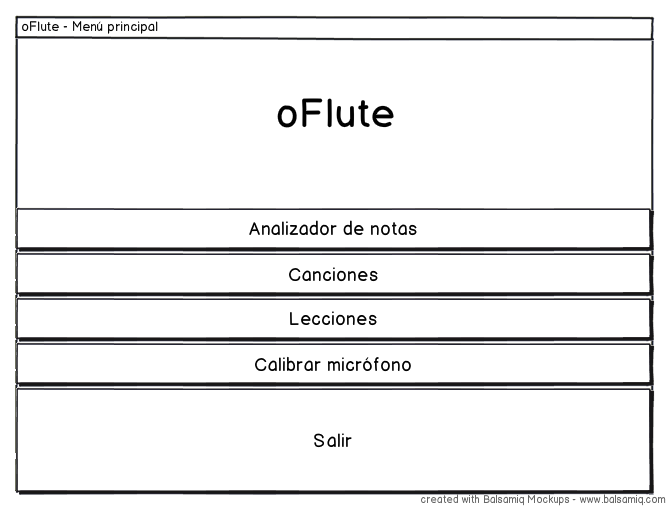
\includegraphics[width=0.6\textwidth]{desarrollo/mockup_menu_principal}
  \caption{Maqueta del menú principal}
\end{figure}

\pagebreak

Las opciones que se incluirán son:
\begin{itemize}
\item \textbf{Analizador de notas}: comprobar las notas que tocamos sobre un
  pentagrama.
\item \textbf{Canciones}: sección principal del juego, en el que aparecerán las
  canciones a tocar.
\item \textbf{Lecciones}: sección de lecciones de aprendizaje.
\item \textbf{Calibrar micrófono}, para ajustarse al nivel de ruido ambiental.
\item \textbf{Salir} al sistema operativo.
\end{itemize}

La siguiente pantalla a modelar será el \textbf{analizador de
  notas}. Simplemente mostrará el logotipo del videojuego a un lado, y un
pentagrama al otro, que se actualizará con la nota detectada por el
micrófono. También contendrá un botón \textit{volver} para ir al menú principal.

\begin{figure}[h!]
  \centering
  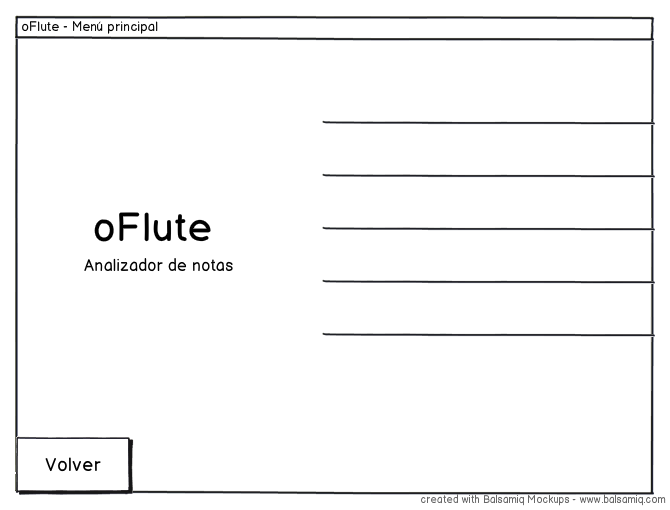
\includegraphics[width=0.6\textwidth]{desarrollo/mockup_analizador}
  \caption{Maqueta de la sección \textit{analizador de notas}}
\end{figure}

La segunda sección a la que se podrá ir desde el menú principal será la de
\textbf{canciones}. Inicialmente, la primera pantalla será la de
\textbf{selección de canción}, que contendrá el logotipo del juego, un botón
para volver al menú principal, y un menú dinámico de canciones que nos permitirá
elegir el tema a interpretar.

\begin{figure}[h!]
  \centering
  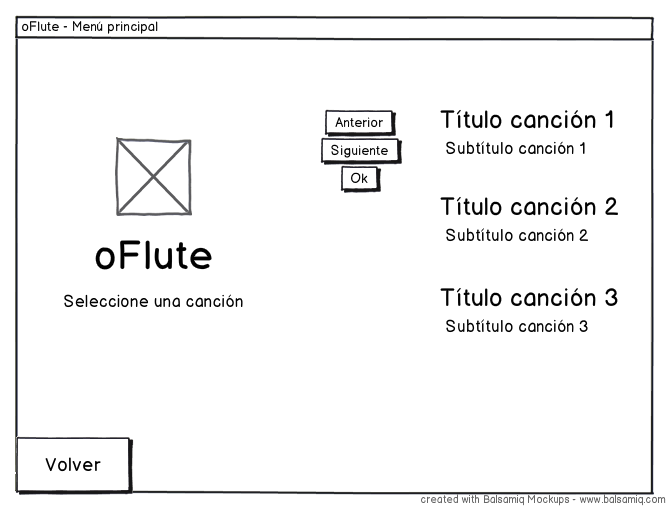
\includegraphics[width=0.6\textwidth]{desarrollo/mockup_seleccionar_cancion}
  \caption{Maqueta del menú de selección de canción}
\end{figure}

Una vez seleccionada la canción, pasaremos a la zona de \textbf{interpretación
  de canción}. Contendrá un pentagrama que ocupará todo el ancho de la pantalla,
con una línea que indicará la zona donde empezar a tocar las notas que
aparezcan. Además, en la parte superior habrá un indicador con la puntuación
obtenida y, abajo, una barra de progreso que nos indicará cuánto queda de
canción.

\begin{figure}[h!]
  \centering
  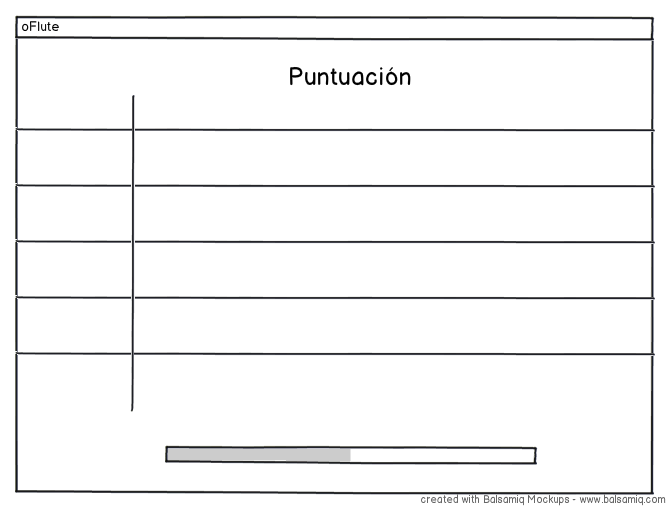
\includegraphics[width=0.6\textwidth]{desarrollo/mockup_reproducir_cancion}
  \caption{Maqueta de la pantalla de interpretación de canción}
\end{figure}

\pagebreak

Al completar la interpretación de la canción, aparecerá la \textbf{sección de
  resultados}. Contendrá el logotipo del juego, el título y subtítulo de la
canción, y un cuadro con información sobre nuestra interpretación, representada
en forma de porcentaje de aciertos. Además, en la zona inferior aparecerá un
mensaje de ánimo dependiendo del resultado obtenido.

\begin{figure}[h!]
  \centering
  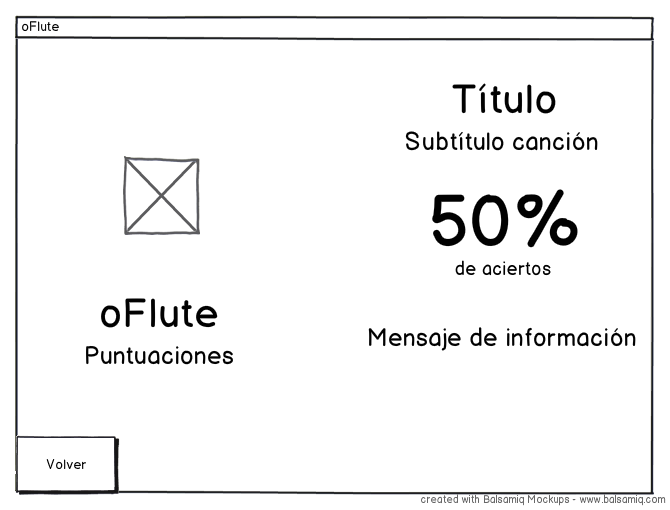
\includegraphics[width=0.6\textwidth]{desarrollo/mockup_puntuaciones}
  \caption{Maqueta de la pantalla de puntuaciones}
\end{figure}

La pantalla de \textbf{selección de lecciones}, a la que se llega desde el menú
principal, contendrá el título, una imagen decorativa, y varios botones para
navegar entre las lecciones cargadas en el sistema. Se mostrará el título y la
descripción de cada lección, así como un botón para comenzar.

\begin{figure}[h!]
  \centering
  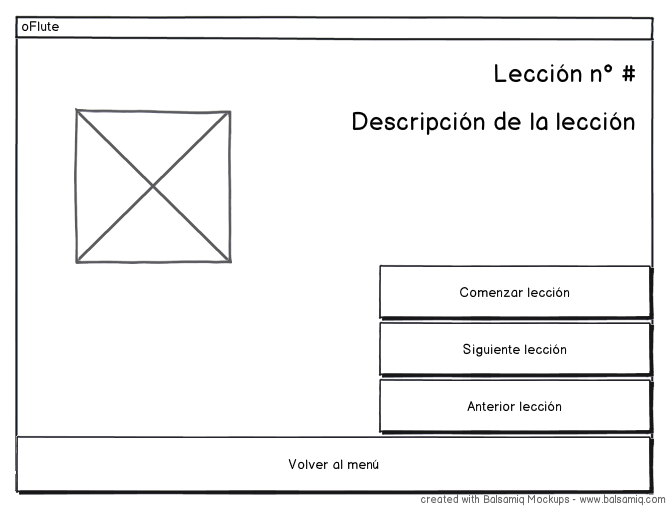
\includegraphics[width=0.6\textwidth]{desarrollo/mockup_seleccionar_leccion}
  \caption{Maqueta del menú de selección de lecciones}
\end{figure}

Una vez elegida una lección, pasaremos a la pantalla de reproducción de
lecciones. Dada la naturaleza \textbf{dinámica} de esta sección, cada lección
podrá tener una apariencia y elementos distintos. El único elemento común entre
todas las lecciones será el botón de \textbf{volver al menú}.

\subsection{Requisitos funcionales}

\textbf{oFlute} se basa en los siguientes requisitos funcionales:
\begin{itemize}
\item Poder terminar la aplicación pulsando el botón de cierre en cualquier
  instante.
\item Comprobar la correcta interpretación de notas individuales mediante el
  analizador de notas.
\item Calibrar el micrófono de forma que el sistema se pueda adaptar al ruido
  ambiental del entorno.
\item Navegar por toda la aplicación de forma sencilla utilizando solo el ratón.
\item Elegir entre varias canciones a interpretar, cada una con su título y
  subtítulo informativos.
\item Interpretar las canciones mediante el uso de la flauta, siguiendo el
  pentagrama en pantalla.
\item Elegir entre bastantes lecciones informativas, poder ejecutarlas y
  seguirlas.
\item Capacidad de añadir nuevas lecciones y canciones de forma sencilla.
\end{itemize}

\subsection{Requisitos de rendimiento}

La aplicación \textbf{oFlute} precisa de unos requisitos bastante básicos,
que en su mayor parte se reducen a cuatro puntos principales:
\begin{itemize}
\item Posesión de una tarjeta de sonido o subsistema de audio similar con un
  micrófono, para poder captar el sonido de la flauta.
\item Pantalla con una resolución de, al menos, 800 por 600 píxeles.
\item Sistema gráfico compatible con OpenGL.
\item Dispositivo apuntador, como un ratón.
\end{itemize}

La práctica totalidad de los ordenadores personales de la actualidad cumplen los
citados requisitos.

\subsection{Requisitos de diseño}
\marginpar{¿?¿?¿?}

\subsection{Requisitos del sistema software}
El sistema de software deberá cumpliar los requisitos siguientes:
\begin{itemize}
\item Deberá funcionar en cualquier sistema \textbf{GNU/Linux} con los
  requisitos anteriormente indicados.
\item Deberá limitarse el número de dependencias, así como facilitar al máximo
  la instalación de las que resultasen imprescindibles.
\item El uso del teclado quedará en segundo plano, haciendo posible utilizar la
  aplicación completamente con el ratón.
\item Al tratarse de un público objetivo juvenil, la aplicación deberá ser
  dinámica, intuitiva y fácil de usar, y la apariencia debe ser agradable.
\item Se evitará el uso de constantes y recursos dentro del código de la
  aplicación, utilizando como alternativa ficheros para representar las
  lecciones y las canciones.
\end{itemize}

\section{Modelo de casos de uso}

A la hora de modelar los casos de uso del sistema, hemos optado por utilizar
notación \textit{UML}, siguiendo los siguientes pasos:
\begin{itemize}
\item Identificación de los usuarios del sistema y sus roles.
\item Para cada rol, determinar las formas de interactuar con el sistema.
\item Creación de casos de uso para los objetivos que debe cumplir la aplicación.
\item Modularización de los casos de usos mediante la implementación de
  relaciones de inclusión o extensión.
\end{itemize}

\subsection{Diagrama de casos de uso}

\begin{figure}[h!]
  \centering
  \includegraphics[width=0.81\textwidth]{desarrollo/diagrama_de_casos_de_uso}
  \caption{Diagrama de casos de uso}
\end{figure}


\subsection{Descripción de los casos de uso}

\subsubsection{Caso de uso: inicio del juego}
\begin{description}
\item [Descripción] Se muestran los créditos del juego, la pantalla de
  presentación, y finalmente el menú principal, desde donde se accederá al
  resto de secciones del juego.
\item [Actores] \jugador.
\item [Precondiciones] Ninguna.
\item [Postcondiciones] Ninguna.
\item [Escenario principal] $\quad$
  \begin{enumerate}
  \item El \jugador\ inicia la aplicación.
  \item El \sistema\ inicializa el subsistema gráfico.
  \item El \sistema\ muestra la pantalla de créditos y la pantalla de
    presentación de la aplicación.
  \item El \sistema\ muestra el menú principal en la pantalla.
  \item El \jugador\ selecciona la opción \textit{Canciones}.
  \item El \sistema\ accede a la pantalla de \textit{Selección de canción}.
  \end{enumerate}
\item[Extensiones --- flujo alternativo] $\quad$
  \begin{description}
  \item [*a] El \jugador\ cierra la ventana.
    \begin{enumerate}
    \item El \sistema\ libera los recursos y sale de la aplicación.
    \end{enumerate}
  \item [4a] El \jugador\ selecciona la opción \textit{Analizador de Notas}.
    \begin{enumerate}
    \item El \sistema\ accede a la pantalla del analizador de notas.
    \end{enumerate}

  \item[4b] El \jugador\ selecciona la opción \textit{Lecciones}.
    \begin{enumerate}
    \item El \sistema\ accede a la pantalla de \textit{Selección de lecciones}.
    \end{enumerate}
  \item[4c] El \jugador\ selecciona la opción \textit{Calibrar micrófono}.
    \begin{enumerate}
    \item El \sistema\ accede a la pantalla de calibración de micrófono.
    \end{enumerate}
  \item [4d] El \jugador\ selecciona la opción Salir.
    \begin{enumerate}
    \item El \sistema\ libera los recursos y sale de la aplicación.\\
    \end{enumerate}
  \end{description}  
\end{description}


\subsubsection{Caso de uso: selección de canción}

\begin{description}
\item [Descripción] Al \jugador\ se le muestra una lista de las canciones
  detectadas, y éste debe elegir entre ellas la que desea interpretar, o volver
  al menú princial.
\item [Actores] \jugador.
\item [Precondiciones] Ninguna.
\item [Postcondiciones] Una canción queda seleccionada.
\item [Escenario principal] $\quad$
  \begin{enumerate}
  \item El \jugador\ accede, desde el menú principal, al panel de selección de canciones.
  \item El \sistema\ busca las canciones dadas de alta en el juego y muestra un menú con las mismas.
  \item El \jugador\ navega entre las canciones listadas y selecciona una de ellas, pulsando finalmente el botón \textit{Ok}.
  \item El \sistema\ carga la canción y pasa a la pantalla de interpretación de canciones.
  \end{enumerate}
\item[Extensiones --- flujo alternativo] $\quad$
  \begin{description}
  \item [*a] El \jugador\ cierra la ventana.
    \begin{enumerate}
    \item El \sistema\ libera los recursos y sale de la aplicación.
    \end{enumerate}
  \item [3a] El \jugador\ selecciona la opción \textit{Volver}.
    \begin{enumerate}
    \item El \sistema\ muestra la animación de cierre y vuelve al menú principal.
    \end{enumerate}
  \end{description}  
\end{description}


\subsubsection{Caso de uso: interpretación de canción}

\begin{description}
\item [Descripción] Tras haber elegido la canción a interpretar, se muestra una
  partitura con las notas que el \jugador\ deberá tocar para conseguir la puntuación deseada.
\item [Actores] \jugador.
\item [Precondiciones] Se ha elegido una canción.
\item [Postcondiciones] Se completa la interpretación de la canción, obteniendo una calificación
\item [Escenario principal] $\quad$
  \begin{enumerate}
  \item El \sistema\ carga la canción, leyendo las notas, y muestra en pantalla,
    mediante animaciones, el marcador de puntos y el pentagrama.
  \item El \sistema\ comienza a mostrar notas en el pentagrama, que van
    deslizándose hacia el lado izquierdo, en el que se encuentra la aguja de
    reproducción, e inicia el análisis del sonido.
  \item El \jugador\, al llegar la nota a la aguja de reproducción, toca la
    flauta con la altura y la duración correcta, de forma que el micrófono sea
    capaz de captar el sonido.
  \item El \sistema\ analiza el sonido que captura el micrófono y detecta la nota que toca el usuario.
  \item El \sistema\ determina que la nota es la correcta y suma los puntos correspondientes.
  \item Mientras existan más notas, se vuelve al punto 2.
  \item El \sistema\ determina que no hay más notas que mostrar, e inicia las
    animaciones para ocultar los elementos en pantalla.
  \item El \sistema\ pasa a la sección de \textit{Resultados de la interpretación}.
  \end{enumerate}
\item[Extensiones --- flujo alternativo] $\quad$
  \begin{description}

  \item [*a] El \jugador\ cierra la ventana.
    \begin{enumerate}
    \item El \sistema\ libera los recursos y sale de la aplicación.
    \end{enumerate}

  \item[*b] El \jugador\ pulsa la tecla \texttt{escape}.
    \begin{enumerate}
    \item El \sistema\ vuelve a la pantalla de \textit{selección de canción}.
    \end{enumerate}

  \item [3a] El \jugador\ toca el instrumento con intensidad insuficiente o nula
    y el sonido no llega al sistema.
    \begin{enumerate}
    \item El \sistema\ representa esta inconsistencia como un silencio.
    \end{enumerate}

  \item [4a] El \sistema\ no es capaz de determinar fehacientemente la nota que
    toca el usuario.
    \begin{enumerate}
    \item El \sistema\ representa esta inconsistencia como un silencio.
    \end{enumerate}

  \item[5a] El \sistema\ determina que la nota tocada por el usuario no es la
    que corresponde a la partitura.
    \begin{enumerate}
    \item El \sistema\ ignora esta situación y no suma los puntos al marcador.
    \end{enumerate}

  \end{description}  
\end{description}

\subsubsection{Caso de uso: resultados de la interpretación}

\begin{description}
\item [Descripción] Después de interpretar las notas de la partitura, se
  muestran los datos obtenidos del análisis de las notas tocadas por el \jugador.
\item [Actores] \jugador.
\item [Precondiciones] Se ha elegido e interpretado una canción.
\item [Postcondiciones] Se completa la partida actual.
\item [Escenario principal] $\quad$
  \begin{enumerate}
  \item El \sistema\ compara la puntuación conseguida con la máxima puntuación
    obtenible, y genera un porcentaje de aciertos.
  \item El \sistema\ muestra, mediante animaciones, un mensaje con información
    sobre la canción y sobre la interpretación del \jugador\, representada
    mediante un porcentaje de aciertos.
  \item El \sistema\ muestra un mensaje variable en función del número de
    aciertos conseguido.
  \item El \jugador\ revisa su puntuación y pulsa el botón \textit{volver} para
    ir de vuelta al menú de \textit{selección de canción}.
  \end{enumerate}
\item[Extensiones --- flujo alternativo] $\quad$
  \begin{description}

  \item [*a] El \jugador\ cierra la ventana.
    \begin{enumerate}
    \item El \sistema\ libera los recursos y sale de la aplicación.
    \end{enumerate}

  \item[4a] El \jugador\ pulsa la tecla \texttt{escape}.
    \begin{enumerate}
    \item El \sistema\ vuelve a la pantalla de \textit{selección de canción}.
    \end{enumerate}

  \end{description}  
\end{description}


\subsubsection{Caso de uso: analizador de notas}

\begin{description}
\item [Descripción] El \jugador\ elige la opción \textit{analizador de notas} en
  el menú principal y es llevado a esta sección, en la que el sistema
  representará gráficamente la nota que esté tocando con la flauta en cada
  instante, sin otra interacción
\item [Actores] \jugador.
\item [Precondiciones] Ninguna.
\item [Postcondiciones] Ninguna
\item [Escenario principal] $\quad$
  \begin{enumerate}
  \item El \jugador\ accede, desde el menú principal, al panel del analizador de notas.
  \item El \sistema\ muestra, mediante animaciones, la pantalla de la sección,
    representada mediante una fracción de partitura en la que se representará la
    nota que esté tocando el \jugador\ en cada momento.
  \item El \sistema\ inicia el análisis del sonido.
  \item El \jugador\ toca la nota que desee con su flauta, de forma que el
    micrófono sea capaz de captar el sonido.
  \item El \sistema\ analiza el sonido que captura el micrófono y detecta la
    nota que toca el usuario.
  \item El \sistema\ muestra en pantalla la nota, sobre la partitura,
    correspondiente a lo que ha tocado el usuario.
  \item Se repite el flujo desde el punto 4, mientras el \jugador\ no pulse en
    el botón volver.
  \item El \jugador\ pulsa en el botón \textit{volver}.
  \item El \sistema\ inicia las animaciones para ocultar los elementos en pantalla.
  \item El \sistema\ vuelve al menú principal.
  \end{enumerate}
\item[Extensiones --- flujo alternativo] $\quad$
  \begin{description}

  \item [*a] El \jugador\ cierra la ventana.
    \begin{enumerate}
    \item El \sistema\ libera los recursos y sale de la aplicación.
    \end{enumerate}

  \item[*b] El \jugador\ pulsa la tecla \texttt{escape}.
    \begin{enumerate}
    \item El \sistema\ vuelve al menú principal.
    \end{enumerate}

  \item [4a] El \jugador\ toca el instrumento con intensidad insuficiente o nula
    y el sonido no llega al sistema.
    \begin{enumerate}
    \item El \sistema\ representa esta inconsistencia como un silencio.
    \end{enumerate}

  \item [5a] El \sistema\ no es capaz de determinar fehacientemente la nota que
    toca el usuario.
    \begin{enumerate}
    \item El \sistema\ representa esta inconsistencia como un silencio.
    \end{enumerate}
  \end{description}  
\end{description}

\subsubsection{Caso de uso: calibración de micrófono}
\begin{description}
\item [Descripción] El \jugador\ elige la opción \textit{calibrar micrófono} en
  el menú principal y es llevado a esta sección, en la que el \sistema\ calibrará
  el micrófono de forma que sea posible aislar el sonido de la flauta del ruido
  ambiental.
\item [Actores] \jugador.
\item [Precondiciones] Ninguna.
\item [Postcondiciones] El \sistema\ obtiene un valor umbral con el que
  discernir entre el sonido del instrumento y el ruido ambiente.
\item [Escenario principal] $\quad$
  \begin{enumerate}
  \item El \jugador\ accede, desde el menú principal, al panel de calibración del micrófono.
  \item El \sistema\ muestra la sección, indicando con un mensaje que el usuario
    debe pulsar la tecla \texttt{escape} para iniciar la calibración.
  \item El \jugador\ pulsa la tecla \texttt{escape} y se mantiene en silencio.
  \item El \sistema\ inicia el análisis del sonido, guardando durante dos
    segundos los valores de ruido que lee del micrófono.
  \item El \sistema\ calcula, a partir de los valores leídos, el umbral de
    ruido, y muestra un mensaje informando del final del proceso.
  \item El \jugador\ pulsa la tecla \texttt{escape} y el \sistema\ vuelve al
    menú principal.
  \end{enumerate}
\item[Extensiones --- flujo alternativo] $\quad$
  \begin{description}

  \item [*a] El \jugador\ cierra la ventana.
    \begin{enumerate}
    \item El \sistema\ libera los recursos y sale de la aplicación.
    \end{enumerate}

  \item[*b] El \jugador\ pulsa la tecla \texttt{escape}.
    \begin{enumerate}
    \item El \sistema\ cancela la calibración y vuelve al menú principal.
    \end{enumerate}

  \item [5a] El \sistema\ encuentra valores inválidos al leer el ruido
    ambiental.
    \begin{enumerate}
    \item El \sistema\ informa al usuario del fallo del proceso de calibración.
    \item El \jugador\ pulsa la tecla \texttt{escape} y el \sistema\ vuelve al
      menú principal.
    \end{enumerate}
  \end{description}  
\end{description}

\subsubsection{Caso de uso: selección de lecciones}
\begin{description}
\item [Descripción] El \jugador\ elige la opción \textit{lecciones} en el menú
  principal y es llevado a esta sección, en la que el \sistema\ mostrará una
  lista de lecciones cargadas, entre las que el usuario deberá elegir.
\item [Actores] \jugador.
\item [Precondiciones] Ninguna.
\item [Postcondiciones] Se ha elegido una lección
\item [Escenario principal] $\quad$
  \begin{enumerate}
  \item El \jugador\ accede, desde el menú principal, al panel de selección de lecciones.
  \item El \sistema\ carga la lista de secciones y muestra, mediante
    animaciones, el panel, preseleccionando por defecto la primera lección.
  \item El \jugador\ utiliza los botones de la sección para elegir una de las
    lecciones, y activarla pulsando \textit{comenzar lección}.
  \item El \sistema\ oculta de forma animada el panel de selección de lecciones.
  \item El \sistema\ lee el fichero \texttt{xml} asociado a la lección indicada,
    cargando los elementos que la componen y las animaciones que se ejecutarán.
  \item El \sistema\ ejecuta las animaciones correspondientes a los elementos
    multimedia de la lección.
  \end{enumerate}
\item[Extensiones --- flujo alternativo] $\quad$
  \begin{description}

  \item [*a] El \jugador\ cierra la ventana.
    \begin{enumerate}
    \item El \sistema\ libera los recursos y sale de la aplicación.
    \end{enumerate}

  \item[2a] El \sistema\ detecta que una de las lecciones leídas no está
    correctamente construída.
    \begin{enumerate}
    \item El \sistema\ informa del error en el \textit{log} del programa y omite
      la carga de esa lección.
    \end{enumerate}

  \item[3a] El \jugador\ pulsa la tecla \texttt{escape}.
    \begin{enumerate}
    \item El \sistema\ vuelve al menú principal.
    \end{enumerate}

  \item[6a] El \jugador\ pulsa la tecla \texttt{escape}.
    \begin{enumerate}
    \item El \sistema\ vuelve al menú de selección de lecciones.
    \end{enumerate}

  \end{description}  
\end{description}

\section{Modelo conceptual de datos}

El modelo conceptual de datos representa, de forma esquemática, las clases que
modelan el sistema y las relaciones que existen entre ellas, además de una
pequeña introducción a su utilidad. 
